\documentclass[twoside]{book}

% Packages required by doxygen
\usepackage{fixltx2e}
\usepackage{calc}
\usepackage{doxygen}
\usepackage[export]{adjustbox} % also loads graphicx
\usepackage{graphicx}
\usepackage[utf8]{inputenc}
\usepackage{makeidx}
\usepackage{multicol}
\usepackage{multirow}
\PassOptionsToPackage{warn}{textcomp}
\usepackage{textcomp}
\usepackage[nointegrals]{wasysym}
\usepackage[table]{xcolor}

% Font selection
\usepackage[T1]{fontenc}
\usepackage[scaled=.90]{helvet}
\usepackage{courier}
\usepackage{amssymb}
\usepackage{sectsty}
\renewcommand{\familydefault}{\sfdefault}
\allsectionsfont{%
  \fontseries{bc}\selectfont%
  \color{darkgray}%
}
\renewcommand{\DoxyLabelFont}{%
  \fontseries{bc}\selectfont%
  \color{darkgray}%
}
\newcommand{\+}{\discretionary{\mbox{\scriptsize$\hookleftarrow$}}{}{}}

% Page & text layout
\usepackage{geometry}
\geometry{%
  a4paper,%
  top=2.5cm,%
  bottom=2.5cm,%
  left=2.5cm,%
  right=2.5cm%
}
\tolerance=750
\hfuzz=15pt
\hbadness=750
\setlength{\emergencystretch}{15pt}
\setlength{\parindent}{0cm}
\setlength{\parskip}{3ex plus 2ex minus 2ex}
\makeatletter
\renewcommand{\paragraph}{%
  \@startsection{paragraph}{4}{0ex}{-1.0ex}{1.0ex}{%
    \normalfont\normalsize\bfseries\SS@parafont%
  }%
}
\renewcommand{\subparagraph}{%
  \@startsection{subparagraph}{5}{0ex}{-1.0ex}{1.0ex}{%
    \normalfont\normalsize\bfseries\SS@subparafont%
  }%
}
\makeatother

% Headers & footers
\usepackage{fancyhdr}
\pagestyle{fancyplain}
\fancyhead[LE]{\fancyplain{}{\bfseries\thepage}}
\fancyhead[CE]{\fancyplain{}{}}
\fancyhead[RE]{\fancyplain{}{\bfseries\leftmark}}
\fancyhead[LO]{\fancyplain{}{\bfseries\rightmark}}
\fancyhead[CO]{\fancyplain{}{}}
\fancyhead[RO]{\fancyplain{}{\bfseries\thepage}}
\fancyfoot[LE]{\fancyplain{}{}}
\fancyfoot[CE]{\fancyplain{}{}}
\fancyfoot[RE]{\fancyplain{}{\bfseries\scriptsize Generated by Doxygen }}
\fancyfoot[LO]{\fancyplain{}{\bfseries\scriptsize Generated by Doxygen }}
\fancyfoot[CO]{\fancyplain{}{}}
\fancyfoot[RO]{\fancyplain{}{}}
\renewcommand{\footrulewidth}{0.4pt}
\renewcommand{\chaptermark}[1]{%
  \markboth{#1}{}%
}
\renewcommand{\sectionmark}[1]{%
  \markright{\thesection\ #1}%
}

% Indices & bibliography
\usepackage{natbib}
\usepackage[titles]{tocloft}
\setcounter{tocdepth}{3}
\setcounter{secnumdepth}{5}
\makeindex

% Hyperlinks (required, but should be loaded last)
\usepackage{ifpdf}
\ifpdf
  \usepackage[pdftex,pagebackref=true]{hyperref}
\else
  \usepackage[ps2pdf,pagebackref=true]{hyperref}
\fi
\hypersetup{%
  colorlinks=true,%
  linkcolor=blue,%
  citecolor=blue,%
  unicode%
}

% Custom commands
\newcommand{\clearemptydoublepage}{%
  \newpage{\pagestyle{empty}\cleardoublepage}%
}

\usepackage{caption}
\captionsetup{labelsep=space,justification=centering,font={bf},singlelinecheck=off,skip=4pt,position=top}

%===== C O N T E N T S =====

\begin{document}

% Titlepage & ToC
\hypersetup{pageanchor=false,
             bookmarksnumbered=true,
             pdfencoding=unicode
            }
\pagenumbering{alph}
\begin{titlepage}
\vspace*{7cm}
\begin{center}%
{\Large Philosophers Protocol }\\
\vspace*{1cm}
{\large Generated by Doxygen 1.8.13}\\
\end{center}
\end{titlepage}
\clearemptydoublepage
\pagenumbering{roman}
\tableofcontents
\clearemptydoublepage
\pagenumbering{arabic}
\hypersetup{pageanchor=true}

%--- Begin generated contents ---
\chapter{Philosophers Example}
\label{index}\hypertarget{index}{}\hypertarget{index_intro}{}\section{Introduction}\label{index_intro}
An implementation example for reader-\/writers protocol, giving priority to readers.

The goal of this example is to
\begin{DoxyItemize}
\item create two or more readers,
\item create a writer
\item simlutate some reads and some writes on shared data following the reader-\/writers protol.
\end{DoxyItemize}

See \hyperlink{rws_8c_abf9e6b7e6f15df4b525a2e7705ba3089}{main } function to run the code.

\begin{DoxyDate}{Date}
06/05/2018 
\end{DoxyDate}
\begin{DoxyVersion}{Version}
0.\+1.\+0 
\end{DoxyVersion}
\begin{DoxyAuthor}{Author}
Luca Parolari 
\end{DoxyAuthor}

\chapter{File Index}
\section{File List}
Here is a list of all documented files with brief descriptions\+:\begin{DoxyCompactList}
\item\contentsline{section}{\hyperlink{read__and__skip_8c}{read\+\_\+and\+\_\+skip.\+c} \\*Main file }{\pageref{read__and__skip_8c}}{}
\end{DoxyCompactList}

\chapter{File Documentation}
\hypertarget{philo_8c}{}\section{philo.\+c File Reference}
\label{philo_8c}\index{philo.\+c@{philo.\+c}}


Main file.  


{\ttfamily \#include $<$stdio.\+h$>$}\newline
{\ttfamily \#include $<$string.\+h$>$}\newline
{\ttfamily \#include $<$sys/types.\+h$>$}\newline
{\ttfamily \#include $<$sys/ipc.\+h$>$}\newline
{\ttfamily \#include $<$sys/sem.\+h$>$}\newline
{\ttfamily \#include $<$signal.\+h$>$}\newline
{\ttfamily \#include $<$errno.\+h$>$}\newline
{\ttfamily \#include $<$unistd.\+h$>$}\newline
{\ttfamily \#include $<$stdlib.\+h$>$}\newline
{\ttfamily \#include \char`\"{}sem.\+h\char`\"{}}\newline
Include dependency graph for philo.\+c\+:
\nopagebreak
\begin{figure}[H]
\begin{center}
\leavevmode
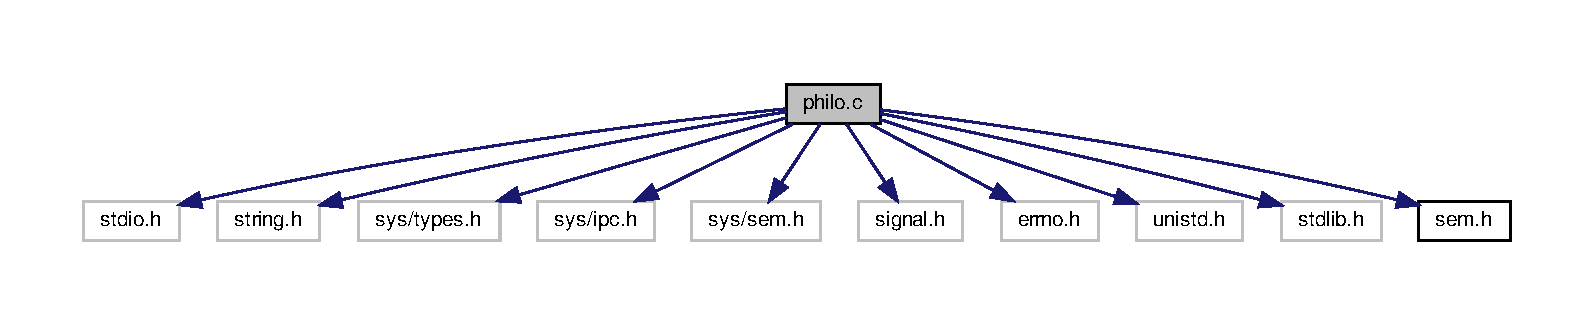
\includegraphics[width=350pt]{philo_8c__incl}
\end{center}
\end{figure}
\subsection*{Functions}
\begin{DoxyCompactItemize}
\item 
int \hyperlink{philo_8c_a5665c342588de1d7d2adeebc24a62afe}{rod1} (int i)
\item 
int \hyperlink{philo_8c_ae669d95f8343b893383e159c064e0263}{rod2} (int i)
\item 
void \hyperlink{philo_8c_a7d74957a358bc5fb34df1bc613cff822}{eat} (int i)
\begin{DoxyCompactList}\small\item\em Simulates eating of the i philosopher. \end{DoxyCompactList}\item 
void \hyperlink{philo_8c_af887e114655ec674ed4eabd1f868223b}{take} (int i)
\begin{DoxyCompactList}\small\item\em Takes the rods. \end{DoxyCompactList}\item 
void \hyperlink{philo_8c_aa0e57b311bb92f0e61d61b52f6bb3803}{place} (int i)
\begin{DoxyCompactList}\small\item\em Places the rods. \end{DoxyCompactList}\item 
void \hyperlink{philo_8c_ae9e5283a5ad8ada1bc570acb676423a0}{philo} (int i)
\begin{DoxyCompactList}\small\item\em Simulates the behaviour of a philosopher. \end{DoxyCompactList}\item 
int \hyperlink{philo_8c_ae66f6b31b5ad750f1fe042a706a4e3d4}{main} ()
\begin{DoxyCompactList}\small\item\em Start a simulation of left-\/handled philosopers protocol. \end{DoxyCompactList}\end{DoxyCompactItemize}
\subsection*{Variables}
\begin{DoxyCompactItemize}
\item 
\mbox{\Hypertarget{philo_8c_aec9fe0a4385efad51521aeaabd33cf74}\label{philo_8c_aec9fe0a4385efad51521aeaabd33cf74}} 
const char \hyperlink{philo_8c_aec9fe0a4385efad51521aeaabd33cf74}{M\+Y\+\_\+\+C\+O\+DE} = \textquotesingle{}a\textquotesingle{}
\begin{DoxyCompactList}\small\item\em Code for generating the I\+PC key. \end{DoxyCompactList}\end{DoxyCompactItemize}


\subsection{Detailed Description}
Main file. 

Implements a philosopher protocol and simulates a context.

\begin{DoxyAuthor}{Author}
L. Parolari 
\end{DoxyAuthor}
\begin{DoxyDate}{Date}
01/06/2018 
\end{DoxyDate}


\subsection{Function Documentation}
\mbox{\Hypertarget{philo_8c_a7d74957a358bc5fb34df1bc613cff822}\label{philo_8c_a7d74957a358bc5fb34df1bc613cff822}} 
\index{philo.\+c@{philo.\+c}!eat@{eat}}
\index{eat@{eat}!philo.\+c@{philo.\+c}}
\subsubsection{\texorpdfstring{eat()}{eat()}}
{\footnotesize\ttfamily void eat (\begin{DoxyParamCaption}\item[{int}]{i }\end{DoxyParamCaption})}



Simulates eating of the i philosopher. 

Simulates eating of the i philosopher printing the start and the end of eating, waiting 5 seconds between start and end. The wait is to simulate some real work with a peripheral device for example. \mbox{\Hypertarget{philo_8c_ae66f6b31b5ad750f1fe042a706a4e3d4}\label{philo_8c_ae66f6b31b5ad750f1fe042a706a4e3d4}} 
\index{philo.\+c@{philo.\+c}!main@{main}}
\index{main@{main}!philo.\+c@{philo.\+c}}
\subsubsection{\texorpdfstring{main()}{main()}}
{\footnotesize\ttfamily int main (\begin{DoxyParamCaption}{ }\end{DoxyParamCaption})}



Start a simulation of left-\/handled philosopers protocol. 

Creates and initializes the mutex and philos semaphores, then starts the philosophers. \mbox{\Hypertarget{philo_8c_ae9e5283a5ad8ada1bc570acb676423a0}\label{philo_8c_ae9e5283a5ad8ada1bc570acb676423a0}} 
\index{philo.\+c@{philo.\+c}!philo@{philo}}
\index{philo@{philo}!philo.\+c@{philo.\+c}}
\subsubsection{\texorpdfstring{philo()}{philo()}}
{\footnotesize\ttfamily void philo (\begin{DoxyParamCaption}\item[{int}]{i }\end{DoxyParamCaption})}



Simulates the behaviour of a philosopher. 

Simulates the think of a philosopher, and after a while the philosopher wakes up and wants to eat. He takes the rod (if he can) then he eat and then he places the rods on the table.


\begin{DoxyParams}{Parameters}
{\em The} & philosopher number \\
\hline
\end{DoxyParams}
\mbox{\Hypertarget{philo_8c_aa0e57b311bb92f0e61d61b52f6bb3803}\label{philo_8c_aa0e57b311bb92f0e61d61b52f6bb3803}} 
\index{philo.\+c@{philo.\+c}!place@{place}}
\index{place@{place}!philo.\+c@{philo.\+c}}
\subsubsection{\texorpdfstring{place()}{place()}}
{\footnotesize\ttfamily void place (\begin{DoxyParamCaption}\item[{int}]{i }\end{DoxyParamCaption})}



Places the rods. 

Places the rods on the table implementing the left-\/handled version of philosophers protocol.


\begin{DoxyParams}{Parameters}
{\em The} & philosopher \\
\hline
\end{DoxyParams}
\mbox{\Hypertarget{philo_8c_a5665c342588de1d7d2adeebc24a62afe}\label{philo_8c_a5665c342588de1d7d2adeebc24a62afe}} 
\index{philo.\+c@{philo.\+c}!rod1@{rod1}}
\index{rod1@{rod1}!philo.\+c@{philo.\+c}}
\subsubsection{\texorpdfstring{rod1()}{rod1()}}
{\footnotesize\ttfamily int rod1 (\begin{DoxyParamCaption}\item[{int}]{i }\end{DoxyParamCaption})}

/return An integer representing the i rod \mbox{\Hypertarget{philo_8c_ae669d95f8343b893383e159c064e0263}\label{philo_8c_ae669d95f8343b893383e159c064e0263}} 
\index{philo.\+c@{philo.\+c}!rod2@{rod2}}
\index{rod2@{rod2}!philo.\+c@{philo.\+c}}
\subsubsection{\texorpdfstring{rod2()}{rod2()}}
{\footnotesize\ttfamily int rod2 (\begin{DoxyParamCaption}\item[{int}]{i }\end{DoxyParamCaption})}

\textbackslash{}/return An integer representing the i+1 rod handled in circular way \mbox{\Hypertarget{philo_8c_af887e114655ec674ed4eabd1f868223b}\label{philo_8c_af887e114655ec674ed4eabd1f868223b}} 
\index{philo.\+c@{philo.\+c}!take@{take}}
\index{take@{take}!philo.\+c@{philo.\+c}}
\subsubsection{\texorpdfstring{take()}{take()}}
{\footnotesize\ttfamily void take (\begin{DoxyParamCaption}\item[{int}]{i }\end{DoxyParamCaption})}



Takes the rods. 

Takes the rods from the table implementing the left-\/handled version of philosophers protocol. The resources taking has hold-\/and-\/wait.


\begin{DoxyParams}{Parameters}
{\em The} & philosopher \\
\hline
\end{DoxyParams}

\hypertarget{sem_8c}{}\section{sem.\+c File Reference}
\label{sem_8c}\index{sem.\+c@{sem.\+c}}


Semaphore sintaxt sugars implementations.  


{\ttfamily \#include $<$stdio.\+h$>$}\newline
{\ttfamily \#include $<$string.\+h$>$}\newline
{\ttfamily \#include $<$sys/types.\+h$>$}\newline
{\ttfamily \#include $<$sys/ipc.\+h$>$}\newline
{\ttfamily \#include $<$sys/sem.\+h$>$}\newline
{\ttfamily \#include $<$signal.\+h$>$}\newline
{\ttfamily \#include $<$errno.\+h$>$}\newline
{\ttfamily \#include $<$unistd.\+h$>$}\newline
{\ttfamily \#include $<$stdlib.\+h$>$}\newline
{\ttfamily \#include \char`\"{}sem.\+h\char`\"{}}\newline
Include dependency graph for sem.\+c\+:
\nopagebreak
\begin{figure}[H]
\begin{center}
\leavevmode
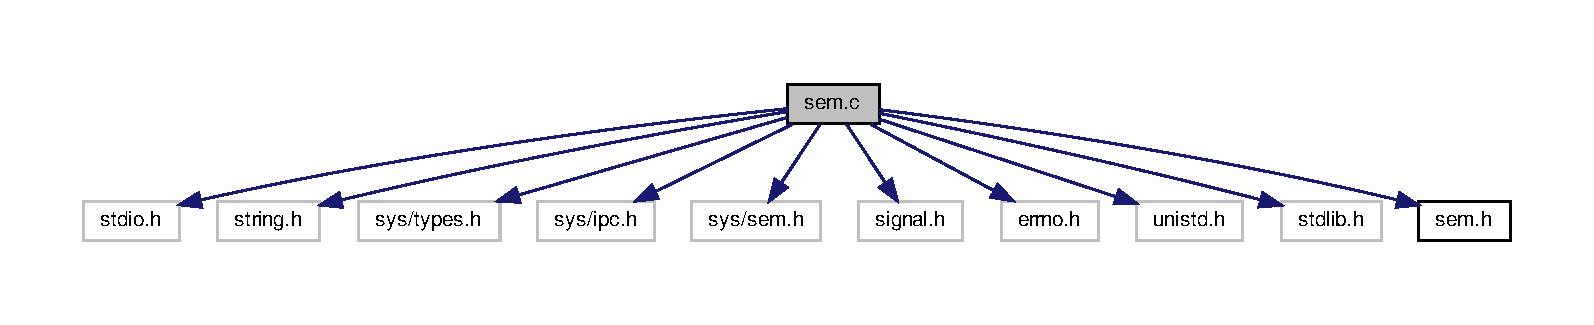
\includegraphics[width=350pt]{sem_8c__incl}
\end{center}
\end{figure}
\subsection*{Functions}
\begin{DoxyCompactItemize}
\item 
void \hyperlink{sem_8c_a7e5e63b16b604bfe1dda13a41b96e4b5}{sem\+\_\+up} (int ipcid, int nsem)
\begin{DoxyCompactList}\small\item\em Dello zucchero sintattico per fare la UP. \end{DoxyCompactList}\item 
void \hyperlink{sem_8c_afa54e0f31b20eb5b3d2b0d6b8aec18b6}{sem\+\_\+down} (int ipcid, int nsem)
\begin{DoxyCompactList}\small\item\em Dello zucchero sintattico per fare la D\+O\+WN. \end{DoxyCompactList}\item 
void \hyperlink{sem_8c_ad4479416be489069e43a17bd246cfe1e}{sem\+\_\+set} (int ipcid, int nsem, int initial)
\begin{DoxyCompactList}\small\item\em Dello zucchero sintattico per impostare il valore di un semaforo. \end{DoxyCompactList}\end{DoxyCompactItemize}
\subsection*{Variables}
\begin{DoxyCompactItemize}
\item 
\mbox{\Hypertarget{sem_8c_a434e4725f04fa366ed1341f04d38521d}\label{sem_8c_a434e4725f04fa366ed1341f04d38521d}} 
const int {\bfseries D\+O\+WN} = -\/1
\item 
\mbox{\Hypertarget{sem_8c_ac58327b7b857c0d4c71c07aa602ace58}\label{sem_8c_ac58327b7b857c0d4c71c07aa602ace58}} 
const int {\bfseries UP} = 1
\end{DoxyCompactItemize}


\subsection{Detailed Description}
Semaphore sintaxt sugars implementations. 

Implements some sintax sugars to easely use semaphores.

Note\+: docs and functions were defined by A. Dal Palù.

\begin{DoxyAuthor}{Author}
L. Parolari 
\end{DoxyAuthor}
\begin{DoxyDate}{Date}
01/06/2018 
\end{DoxyDate}


\subsection{Function Documentation}
\mbox{\Hypertarget{sem_8c_afa54e0f31b20eb5b3d2b0d6b8aec18b6}\label{sem_8c_afa54e0f31b20eb5b3d2b0d6b8aec18b6}} 
\index{sem.\+c@{sem.\+c}!sem\+\_\+down@{sem\+\_\+down}}
\index{sem\+\_\+down@{sem\+\_\+down}!sem.\+c@{sem.\+c}}
\subsubsection{\texorpdfstring{sem\+\_\+down()}{sem\_down()}}
{\footnotesize\ttfamily void sem\+\_\+down (\begin{DoxyParamCaption}\item[{int}]{ipcid,  }\item[{int}]{nsem }\end{DoxyParamCaption})}



Dello zucchero sintattico per fare la D\+O\+WN. 


\begin{DoxyParams}{Parameters}
{\em ipcid} & Riceve il numero dell`oggetto I\+PC \\
\hline
{\em nsem} & Il semaforo su cui fare D\+O\+WN\\
\hline
\end{DoxyParams}
Questa chiamata maschera i dettagli implementativi sul buffer delle operazioni I\+PC \mbox{\Hypertarget{sem_8c_ad4479416be489069e43a17bd246cfe1e}\label{sem_8c_ad4479416be489069e43a17bd246cfe1e}} 
\index{sem.\+c@{sem.\+c}!sem\+\_\+set@{sem\+\_\+set}}
\index{sem\+\_\+set@{sem\+\_\+set}!sem.\+c@{sem.\+c}}
\subsubsection{\texorpdfstring{sem\+\_\+set()}{sem\_set()}}
{\footnotesize\ttfamily void sem\+\_\+set (\begin{DoxyParamCaption}\item[{int}]{ipcid,  }\item[{int}]{nsem,  }\item[{int}]{initial }\end{DoxyParamCaption})}



Dello zucchero sintattico per impostare il valore di un semaforo. 


\begin{DoxyParams}{Parameters}
{\em ipcid} & Riceve il numero dell`oggetto I\+PC \\
\hline
{\em nsem} & Il semaforo da impostare \\
\hline
{\em initial} & Il valore iniziale del semaforo\\
\hline
\end{DoxyParams}
Questa chiamata maschera i dettagli implementativi sul buffer delle operazioni I\+PC \mbox{\Hypertarget{sem_8c_a7e5e63b16b604bfe1dda13a41b96e4b5}\label{sem_8c_a7e5e63b16b604bfe1dda13a41b96e4b5}} 
\index{sem.\+c@{sem.\+c}!sem\+\_\+up@{sem\+\_\+up}}
\index{sem\+\_\+up@{sem\+\_\+up}!sem.\+c@{sem.\+c}}
\subsubsection{\texorpdfstring{sem\+\_\+up()}{sem\_up()}}
{\footnotesize\ttfamily void sem\+\_\+up (\begin{DoxyParamCaption}\item[{int}]{ipcid,  }\item[{int}]{nsem }\end{DoxyParamCaption})}



Dello zucchero sintattico per fare la UP. 


\begin{DoxyParams}{Parameters}
{\em ipcid} & Riceve il numero dell`oggetto I\+PC \\
\hline
{\em nsem} & Il semaforo su cui fare UP\\
\hline
\end{DoxyParams}
Questa chiamata maschera i dettagli implementativi sul buffer delle operazioni I\+PC 
\hypertarget{sem_8h}{}\section{sem.\+h File Reference}
\label{sem_8h}\index{sem.\+h@{sem.\+h}}


Semaphore sintaxt sugars.  


This graph shows which files directly or indirectly include this file\+:
\nopagebreak
\begin{figure}[H]
\begin{center}
\leavevmode
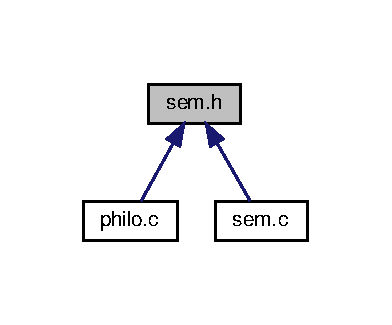
\includegraphics[width=188pt]{sem_8h__dep__incl}
\end{center}
\end{figure}
\subsection*{Functions}
\begin{DoxyCompactItemize}
\item 
void \hyperlink{sem_8h_a7e5e63b16b604bfe1dda13a41b96e4b5}{sem\+\_\+up} (int ipcid, int nsem)
\begin{DoxyCompactList}\small\item\em Dello zucchero sintattico per fare la UP. \end{DoxyCompactList}\item 
void \hyperlink{sem_8h_afa54e0f31b20eb5b3d2b0d6b8aec18b6}{sem\+\_\+down} (int ipcid, int nsem)
\begin{DoxyCompactList}\small\item\em Dello zucchero sintattico per fare la D\+O\+WN. \end{DoxyCompactList}\item 
void \hyperlink{sem_8h_ad4479416be489069e43a17bd246cfe1e}{sem\+\_\+set} (int ipcid, int nsem, int initial)
\begin{DoxyCompactList}\small\item\em Dello zucchero sintattico per impostare il valore di un semaforo. \end{DoxyCompactList}\end{DoxyCompactItemize}


\subsection{Detailed Description}
Semaphore sintaxt sugars. 

Declare some sintax sugars to easely use semaphores.

Note\+: docs and functions were defined by A. Dal Palù.

\begin{DoxyAuthor}{Author}
L. Parolari 
\end{DoxyAuthor}
\begin{DoxyDate}{Date}
01/06/2018 
\end{DoxyDate}


\subsection{Function Documentation}
\mbox{\Hypertarget{sem_8h_afa54e0f31b20eb5b3d2b0d6b8aec18b6}\label{sem_8h_afa54e0f31b20eb5b3d2b0d6b8aec18b6}} 
\index{sem.\+h@{sem.\+h}!sem\+\_\+down@{sem\+\_\+down}}
\index{sem\+\_\+down@{sem\+\_\+down}!sem.\+h@{sem.\+h}}
\subsubsection{\texorpdfstring{sem\+\_\+down()}{sem\_down()}}
{\footnotesize\ttfamily void sem\+\_\+down (\begin{DoxyParamCaption}\item[{int}]{ipcid,  }\item[{int}]{nsem }\end{DoxyParamCaption})}



Dello zucchero sintattico per fare la D\+O\+WN. 


\begin{DoxyParams}{Parameters}
{\em ipcid} & Riceve il numero dell`oggetto I\+PC \\
\hline
{\em nsem} & Il semaforo su cui fare D\+O\+WN\\
\hline
\end{DoxyParams}
Questa chiamata maschera i dettagli implementativi sul buffer delle operazioni I\+PC \mbox{\Hypertarget{sem_8h_ad4479416be489069e43a17bd246cfe1e}\label{sem_8h_ad4479416be489069e43a17bd246cfe1e}} 
\index{sem.\+h@{sem.\+h}!sem\+\_\+set@{sem\+\_\+set}}
\index{sem\+\_\+set@{sem\+\_\+set}!sem.\+h@{sem.\+h}}
\subsubsection{\texorpdfstring{sem\+\_\+set()}{sem\_set()}}
{\footnotesize\ttfamily void sem\+\_\+set (\begin{DoxyParamCaption}\item[{int}]{ipcid,  }\item[{int}]{nsem,  }\item[{int}]{initial }\end{DoxyParamCaption})}



Dello zucchero sintattico per impostare il valore di un semaforo. 


\begin{DoxyParams}{Parameters}
{\em ipcid} & Riceve il numero dell`oggetto I\+PC \\
\hline
{\em nsem} & Il semaforo da impostare \\
\hline
{\em initial} & Il valore iniziale del semaforo\\
\hline
\end{DoxyParams}
Questa chiamata maschera i dettagli implementativi sul buffer delle operazioni I\+PC \mbox{\Hypertarget{sem_8h_a7e5e63b16b604bfe1dda13a41b96e4b5}\label{sem_8h_a7e5e63b16b604bfe1dda13a41b96e4b5}} 
\index{sem.\+h@{sem.\+h}!sem\+\_\+up@{sem\+\_\+up}}
\index{sem\+\_\+up@{sem\+\_\+up}!sem.\+h@{sem.\+h}}
\subsubsection{\texorpdfstring{sem\+\_\+up()}{sem\_up()}}
{\footnotesize\ttfamily void sem\+\_\+up (\begin{DoxyParamCaption}\item[{int}]{ipcid,  }\item[{int}]{nsem }\end{DoxyParamCaption})}



Dello zucchero sintattico per fare la UP. 


\begin{DoxyParams}{Parameters}
{\em ipcid} & Riceve il numero dell`oggetto I\+PC \\
\hline
{\em nsem} & Il semaforo su cui fare UP\\
\hline
\end{DoxyParams}
Questa chiamata maschera i dettagli implementativi sul buffer delle operazioni I\+PC 
%--- End generated contents ---

% Index
\backmatter
\newpage
\phantomsection
\clearemptydoublepage
\addcontentsline{toc}{chapter}{Index}
\printindex

\end{document}
